\subsubsection{Unterirdisches Fahrradparkhaus}
Unterirdische Fahrradparkhäuser sind ein aktueller Trend. Besonders verbreitet sind sie in den Niederlanden, wo sehr großzügig in die Fahrradinfrastruktur investiert wird. Die Vorteile von einem Fahrradparkhaus sind die multiplen Verwendungszwecke, zum Beispiel kann eine Reparaturstation integriert werden.

\noindent Der Nachteil ist, dass sie keinen großen Mehrwert gegenüber einem klassischen Fahrradständer oder einer Fahrradbox bieten, da zwar ein Schutz gegenüber den Umwelteinflüssen wie Regen und Schnee besteht, jedoch Vandalismus trotzdem möglich ist. Ein wesentlicher Nachteil sind die hohen Baukosten für ein entsprechendes Gebäude.

\begin{figure}[H]
    \centering
    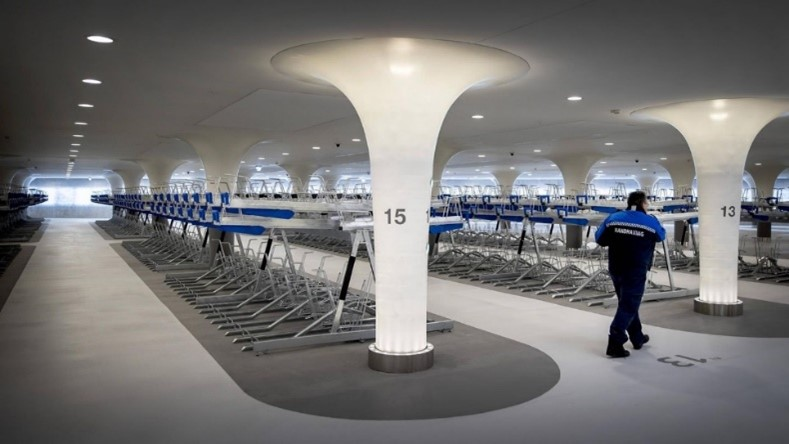
\includegraphics[width=0.5\textwidth]{images/unterirdischesfahrradparkhaus.jpg}
    \caption{Fahrrad-Tiefgarage in Amsterdam \citev{fahradtiefgarage}}
    \label{fig:fahradtiefgarage}
\end{figure}

\noindent Die Abbildung \ref{fig:fahradtiefgarage} zeigt ein unterirdisches Parkhaus in Amsterdam. Die Baukosten des Gebäudes betragen 60 Millionen Euro. Es bietet Platz für 11.000 Fahrräder.
